% !TEX root = /home/fred-olav/afgv/src/preamble.tex
% Start preamble
\documentclass[10pt,a5paper]{article}
\usepackage{geometry}
 \geometry{
 a5paper,
 total={120mm,185mm},
 left=10mm,
 top=10mm,
 }
\usepackage[utf8]{inputenc}
\usepackage[T1]{fontenc}
\usepackage[pdftex]{graphicx}
\graphicspath{{./}}
\usepackage{enumitem}
\usepackage{pdfpages}
\usepackage{hyperref}
\usepackage{tikz}
\usepackage{attachfile}
\usepackage[ngerman]{babel}
\usepackage{epstopdf}
\usepackage{array}
\usepackage{longtable}
\usepackage{amsmath}
\usepackage{makecell}
%\usepackage[table]{xcolor,colorbl}
%\setlength{\textwidth}{11cm}
%\setlength{\oddsidemargin}{-0.5cm}
\setlength{\evensidemargin}{-1.5cm}
%\setlenght{\headsep}{0cm}
\setlength\parindent{0pt}
%\setlength{\extrarowheight}{3pt}
\usepackage{listings}
\usepackage{microtype}
%\usepackage{xcolor}

\input{../src/arduinoLanguage.tex}

\include{def}
% End preamble

\begin{document}
\huge
\centerline \textbf{Håndbok for 3AUA Gand VGS} \bigskip
\normalsize
\vfil \eject
\section {Utførelse av arbeidsoppdrag}
%Måleteknikk 
\hrule

\vskip 1cm

I 3AUA utføres praktisk arbeid som arbeidsoppdrag, disse skal bestå av følgende:\begin{itemize}[noitemsep]
	\item Planlegging
	\item Gjennomføring
	\item Dokumentasjon
\end{itemize}

\subsection {Planlegging}

Planleggingen av arbeidsoppdragene har som hensikt å:

\begin{itemize}[noitemsep]
	\item Sørge for at vi har kunnskap nok til å starte opp arbeidet. 
	\item Tenke igjennom hva arbeidet består av og i hvilken rekkefølge det er hensiktmessig å utføre det. 
	\item Sørge for av vi har alt nøvendig utstyr og materiell. 
\end{itemize}



Alt arbeid skal risikovurderes utførelse. Nødvendig sikringstiltak skal planlegges og utføres i henhold til bedriftens HMS-regelverk. Eksempelvis skal all energitilførsel stenges og sikres mot utilsiktet innkopling, hvis mulig. Hvis ikke, skal arbeidene planlegges og utføres under gjeldende sikringstiltak, eksempelvis med AUS verktøy isolerende matter, etc. Husk spesielt personlig verneutstyr, så som briller, hjelm, hansker, sko, klær, hørselvern, etc.

Planleggingsdlen skal innholde:\begin{itemize}[noitemsep]
	\item Din forståelse av oppgaven
	\item 
\end{itemize}

Fremdriftsplan:
\vskip 5pt 
Skal vise at du forstår hva som inngår av arbeid i de ulike oppdragene og at du forstår i hvilken rekkefølge de må utføres. Denne er også et greit utgangpunkt for å hvilke deler som sakl være med i en risikovurdering. 

\vskip 5pt 
Risikovurdering:
\vskip 5pt 
Skal vise at du kan vurdere farer med arbeidet og sette inn tiltakt for å unngå farene. FSE er sentral i forhold til farer med elektrisitet. 

\vskip 5pt 
SJA skal utføres om et arbeid ikke er kjent eller det finnes rutine for det. Som elev i et fag vil det si at i de flese arbeidsoppdrag må det utføres en SJA. 
\vskip 5pt 
Verktøysliste:
\vskip 5pt 
Skal vise at du vet hvilket verktøy som trengs til de ulike jobbene. Å bruke korrekt navn er en viktig del. 
\vskip 5pt 

Utstyrsliste:
\vskip 5pt 
Skal vise at du vet hvilket utstyr som trengs til de ulike jobbene. Å bruke korrekt navn er en viktig del. Utstyrslisten skal inneholde det som du ville tatt betalt for av en kunde. 

\vskip 10pt 
Teori, vuderinger og beregninger. 


\vskip 10pt 
\subsection{Gjennomføring}

Enten arbeidsoppdraget skal utføres i praksis eller det bare er en del av en prøve skal gjennomføringenen beskrives. Dette er viktig del øvelsen til å besvare eksamensoppgaver. 
\vskip 5pt 
Om du har utført arbeidet kan det være lurt å beskrive hvordan du ville utført arbeidet om du skulle gjort det en gang til. 
\subsection{Dokumentasjon}

\vskip 5pt 
Alle arbeidsoppdrag skal inneholde relevant dokumentajson i forhold til arbeidet som er gjort. Det kan f.eks. være et prosjekt der du må levere komplett dokumentajson. Et annet eksempel kan være kalibrering av en transmitter der en kort arbeidsrapport og et kalibreringsskjema vil være relevant. 




\vfil \eject
\section{Kapittel 2 - Dokumentasjon}
\subsection{Instrument identifiserings tag} 

Frem til nå har vi sett på flere typer instrument skjema, i alle har de for skjellige instrumentene hatt en kode som forklarer funksjonen. TT er en Termperatur Transmitter, PDT er en Trykk Differanse Transmitter eller FV er en Flow Ventil. Disse bokstavene er definert i ISO 14617-6. 

\vskip 5pt 
Hvert instrument i et automatisert anlegg bør ha sin egen unike \textit{tag}, bestående av en bokstavkode som beskriver instrumentet sin funksjon i tillegg til et tall som beskriver hvilken sløyfe det tilhører. Det kan også være nummer som referer til et større om område i anlegget. Det samme instrumentet kan brukes flere plasser i en sløyfe, en kan da bruke en bokstavkode til de ulike delene.  

\vskip 5pt 
Som et eksempel, hvis vi ser et instrument med tag\texttt{FC-135}, så vet vi at det er en \textit{flow controller} (FC) for sløyfe 135. I et stort prosessanlegg med flere områder med ulike funksjoner, ville kanskje dette instrumentet vært merket 12-FC-135 (flow controller for sløyfe 135 i område 12. ) Om denne støyfen inneholdt flere regulatorer (controllere), kunne skilt mellom dem ved å bruke etterfølgende bokstaver på sløyfenummeret. (12-FC-135A, 12-FC-135B, 12-FC-135C). 

\vskip 5pt 
Alle instrumenter i en sløyfe blir identifisert med en bokstav som beskriver variabelen som sløyfen skal regulere, helt uavhengig av den fysike oppbygning av instrumentet. Vår tenkte flow controller FC-135, kan være fysisk lik nivå regulatoren i sløyfe \#72 (LC-72), eller til temperatur regulatoren i sløyfe \#288 (TC-288). Det som gjør FC-135 til en strømningsregulator er at den primære variabelen den skal regulere er strømning. Alle andre instrumenter i denne sløyfen vil også ha F som første bokstav\footnote{Exceptions do exist to this rule.  For example, in a cascade or feedforward loop where multiple transmitters feed into one or more controllers, each transmitter is identified by the type of process variable \textit{it} senses, and each controller's identifying tag follows suit.}. I en nivåreguleringssøyfe kan dette se slik ut: Transmitteren merkes "LT" selv om den måler trykk for å angi nivå, regulatoren merkes "LC" og reguleringsventilen merkes LV selv om den i prakses justerer strømning. Dette fordi deres primære funksjon er å bidra til nivåregulering. 


\vskip 5pt 
Bokstaver som kan brukes til å identifisere instrumenter angis i standarder. ISO14617-6 er en slik standard. Det finnes flere standarder i bruker rundt om i verden og gamle anlegg kan være basert på eldre standarder. Tabellen nedenfor er et utdrag av vanlige bokstaver som brukes. Legg merke til at bruken av signalomformer definerer en unik variabel. f.eks. en "PT" er en trykktransmitter som måler trykk på en plass, mens "PDT" er en måling av trykkdifferanse mellom to punkter. På samme måte kan "TC" være en temperaturregulator som regulerer temperaturen i en prosess, mens "TKC" er en regulator som regulerer temperatur forandring. 

% No blank lines allowed between lines of an \halign structure!
% I use comments (%) instead, so that TeX doesn't choke.
\hrule
\small
\begin{center}
\begin{tabular}{ | m{1cm} | m{2.5cm}| m{2cm} | m{2.5cm} |} 
\hline
\multicolumn{4}{|c|}{Bokstavkode for indentifisering av instrumentfunksjoner} \\
\hline
	Bokst. & Variabel& Omformer & Funksjon \\ 
\hline
	A&&&Alarm\\
\hline
	B&&&Visning av diskre status\\
\hline
	C&&&Regulerende\\
\hline
	D&Densitet&Differanse&\\
\hline
	E&Elektrisk variabel&&Elemens (følende)\\
\hline
	F&Flow rate&Forhold&\\
\hline
	G&Posisjon, lengde&&Visning\\
\hline
	H&Håndbetjent&&\\
	\hline
	I&&&Indikerende\\
	\hline
	J&Effekt&Avsøke&\\
	\hline
	K&Tid&Forandring i tid&\\
	\hline
	L&Nivå&&\\
	\hline
	M&Fuktighet eller Relativ fuktighet&&\\
	\hline
	N&Etter brukers valg&&\\
	\hline
	N&Etter brukers valg&&\\
	\hline
	P&Trykk eller vakum&&Tilkobling til testpunkt\\
	\hline
	Q&\makecell{Egenskap\\f.eks:\\*Analyse\\*Konsentrasjon}&Integrere eller summere&Integrerende eller summerende\\
	\hline
	R&Radioaktiv stråling&&Skrivende\\
	\hline
	S&Hastighet&&Bryterfunksjon\\
	\hline
	T&Temperatur&&Overføring\\
	\hline
	U&Multivariabel&&Multifunksjon\\
	\hline
	V&Etter brukers valg& &Påvirkning på prosess med ventil eller pumpe, o.l.\\
	\hline
	W&Vekt, Kraft&Multipliserende&\\
	\hline
	X&Uspesifiserte variabler&&Uspesifisert\\
	\hline
	Y&Etter brukers valg&&Konvertering eller algoritme\\
	\hline
	Z&Antall hendelser, antall&&Nødbetjening eller sikkerhetsfunksjon\\
\hline
\end{tabular}
\end{center}
\normalsize
%Måleteknikk 
\vskip 5pt
\hrule

\vskip 5pt

\subsection{Referansebetegnelsessystem}
\small
\begin{center}
\begin{tabular}{ | m{1cm} | m{2.5cm}| m{2cm} | m{2.5cm} |} 
\hline
\multicolumn{4}{|c|}{Bokstavkode for utstyri} \\
\hline
	Bokst. & Variabel& Omformer & Funksjon \\ 
\hline
	A&&&Alarm\\
\hline
	B&Sensorer&&Visning av diskre status\\
\hline
	C&Lagring&&Regulerende\\
\hline
	E&Strålende objekt&&\\
\hline
	F&Beskyttende objekt&&\\
\hline
	G&Beskyttende objekt&&\\
\hline
	H&Prossesring av materie&&\\
	\hline
	K&Prosessring av informasjon&&\\
	\hline
	L&Nivå&&\\
	\hline
	M&Objekt som driver noe&&\\
	\hline
	N&&&\\
	\hline
	P&objekt som presenterer&&\\
	\hline
	Q&objekt som presenterer&&\\
	\hline
	R&Objekt som begrenser&&\\
	\hline
	S&Objekt for betjening &&\\
	\hline
	T&Transformerende objekt&&\\
	\hline
	U&Objekt som holder&&\\
	\hline
	W&Førende objekt&&\\
	\hline
	X&Objekt for overgang&&\\
	\hline
\hline
\end{tabular}
\end{center}
\normalsize
%Måleteknikk 
\vfil \eject
\subsection{Symboler}
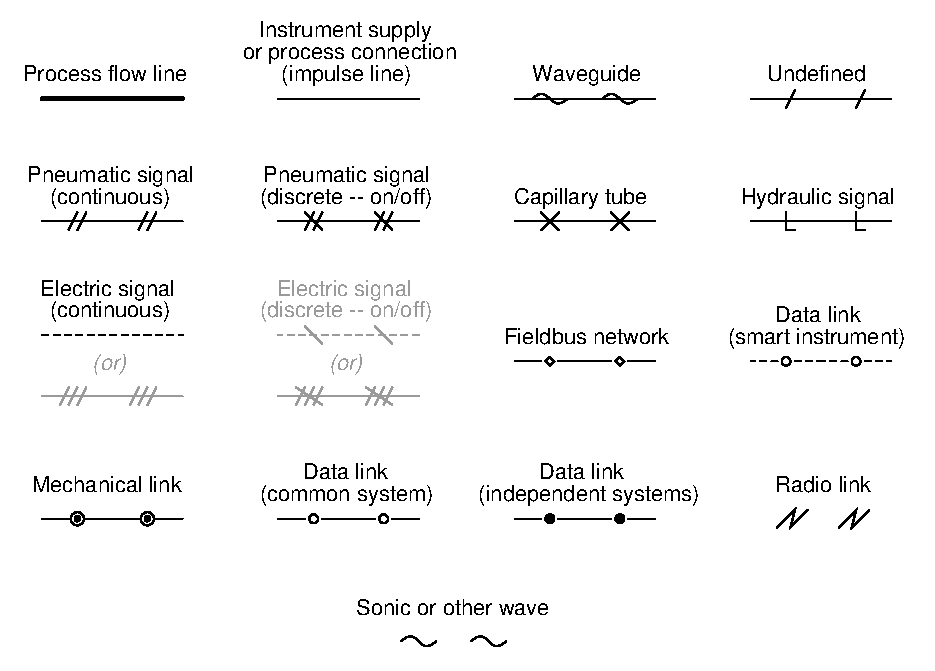
\includegraphics[width=1\textwidth]{diagrams00.eps}
\includegraphics[width=1\textwidth]{diagrams01.eps}
\includegraphics[width=1\textwidth]{diagrams02.eps}
\includegraphics[width=1\textwidth]{diagrams03.eps}
\includegraphics[width=1\textwidth]{diagrams04.eps}
\includegraphics[width=1\textwidth]{diagrams05.eps}
\includegraphics[width=1\textwidth]{diagrams06.eps}
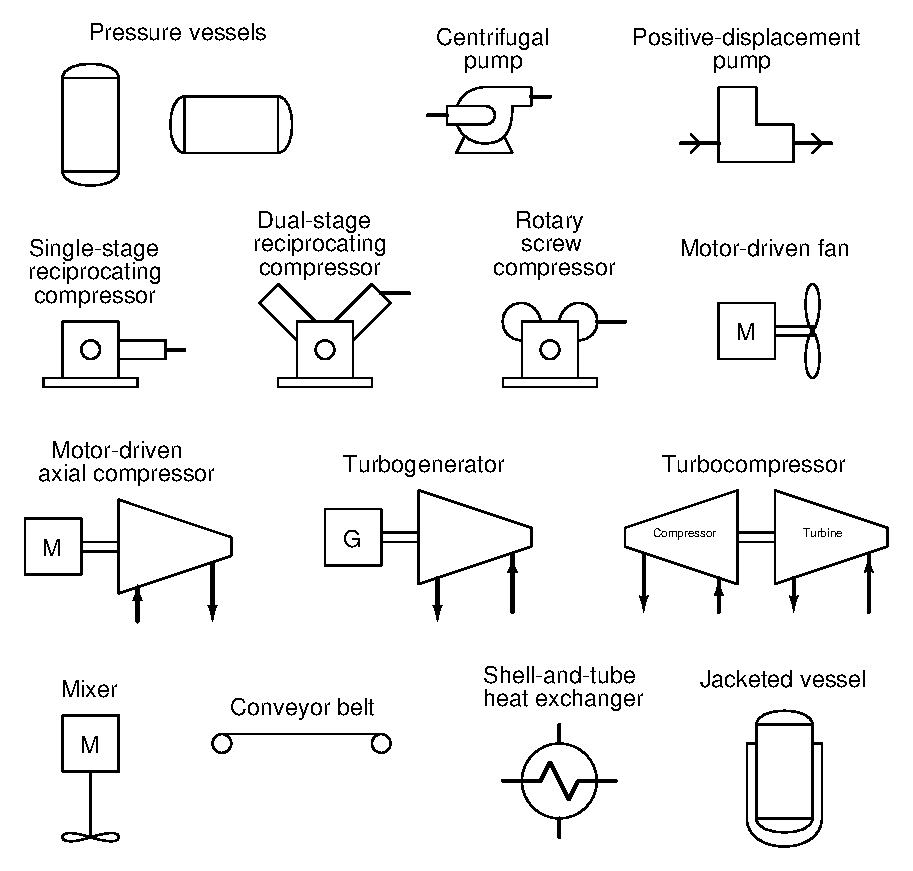
\includegraphics[width=1\textwidth]{diagrams07.eps}
\includegraphics[width=1\textwidth]{diagrams10.eps}
\includegraphics[width=1\textwidth]{diagrams11.eps}
\includegraphics[width=1\textwidth]{diagrams12.eps}
\includegraphics[width=1\textwidth]{diagrams13.eps}
\includegraphics[width=1\textwidth]{diagrams14.eps}
\textbf{Kapittel 3 - Instrumentering}
%Måleteknikk

\begin{center}
\begin{longtable}{ | m{2cm} | m{7cm} | } 
\hline
\multicolumn{2}{|c|}{Definisjoner} \\
\hline
Begrep	& Beskrivelse \\ 
\hline
\hline
	Avvik&Forskjellen mellom den målte verdien og ønsket verdi (skalverdi) i ei reguleringssløyfe\\
	\hline
	Dødgang (dødsone)&For prosessinstrumenter er dødgang det området som et inngangssignal kanforandres innenfor, uten at det vises noen forandring i utgangssignalet. Med forandring menes her reversering av retningen på inngangssignalet\\
	\hline
	Forsterkning&Forholdet mellom forandring i inngangsverdien i forhold til den utgangsverdien som var årsak til forandringen\\
	\hline
	Hysterese&Samme måleverdi kan gi ulike utsignaler fra måleomformeren ved samme verdi, Hysterese oppstår når måleverdien veksler mellom å være stigende eller fallende.\\
	\hline
	Kalibrering&Sjekk av at måleinstrumentets verdier stemmer med et intrument med høyere nøyaktihet. Noen intrumenter kan justeres inn om de ikke stemmer overens.\\ 
	\hline
	Lesbarhet&Den minste inndeling på skalaen på et instrument.\\
	\hline
	Måleomfang&Differansen mellom øvre og nedre målegrense\\
	\hline
	Målegrense&URV: høyeste verdi som instrumentet kan vise. LRV: laveste verdi som instrumentet kan vise. \\
	\hline
	Målegrense&Den fulle skalaen for en måling, indikering eller avlesning. Eksempelvis -50 til 150°C\\
	\hline
	Nullpunktfeil&En forskyving av nede målegrense\\
	\hline
	Nøyaktighet& Forskjell mellom avlest og virkelig verdi for en målt variabel.\\
	\hline

	Reproduser- barhet& Evnen til å reprodusere samme resultat fra en rekke uavhengige målinger av den samme verdien selv om målingen utføres av forskjellige personer, på forskjellige steder og under ulike klimatiske forhold.\\
	\hline
	Repeterbarhet&Samsvar mellom en rekke på hverandre følgende målinger av utgangsverdi for den samme inngangsverdien. Målingene foretas under samme klimatiske forhold, av samme person og med korte intervaller.\\
	\hline
	Ulinearitet&En type feil der inngangsverdiene til et instrument ikke forholder seg til den ideelle rettlinjede sammenhengen mellom inngangs- og utgangs-verdiene (referansekarakteristikken).\\
	\hline

Regulator & En enhet som har til oppgave å påvirke prosessen slik at den oppnår en ønsket tilstand (f.eks. et ønsket nivå eller en ønsket temperatur).\\
	\hline
Prosess & Det anlegget eller systemet som inngår i reguleringen.\\
	\hline
Prosessvariabel & Den fysiske størrelsen i prosessen som skal reguleres (nivå, trykk, temperatur etc.)\\
	\hline
ProsessVerdi PV & Den verdien prosessvariabelen til enhver tid har.\\
	\hline
Settpunkt SP & Den verdien vi ønsker at prosessvariabelen skal ha.\\
	\hline
Manipulerende Variabel MV & Signalet som styrer pådragsorganet\\
	\hline
Forsyning & \\
	\hline
Pådrag & Det som er ment å variere prosessvariabelen. F.eks. væske inn i en nivåtank. \\
	\hline
Belastning & Det som tas ut av prosessen ved konstant PV. Vil ha samme verdi som pådraget. \\
	\hline
Forstyrrelse & Forandringer som påvirker verdien til prosessvariabelen. \\
	\hline
Avviket e & Forskjellen mellom PV og SP (Direkte virkning PV-SP, Reverserende virkning SP-PV)\\
	\hline
Pådragsorgan & Den komponenten som styrer pådraget (f.eks. motoren i bilen som påvirker hastigheten, eller ventilen som påvirker nivået i tanken).\\
	\hline
Forstillingsenhet & I vårt eksempel med regulering av bilens hastighet, er forstillingsenheten forgasseren. Motoren er pådragsorganet i reguleringssløyfen.\\
	\hline
Auto og Manuell modus (Lukket& eller åpensløyfe). Om pådraget styres av regulatoren eller en manuell innstilt verdi. \\
	\hline
LRV og URV& ( Lover Range Value og Upper Range value, Laveste og høyeste verdi målesignalet kan ha.)\\

	\hline


\end{longtable}
\end{center}
\vskip 5pt
\hrule

\vskip 5pt

\subsubsection{skallering}
$$\includegraphics{current63.eps}$$

Ut fra denne representasjonen kan vi sette opp følgende formel for konvertering mellom signaler. 
$$		\frac{y-y_{start}}{y_{range}}=\frac{x-x_{start}}{x_{range}}$$

$$\includegraphics{current59.eps}$$
\vfil \eject
\section{Reguleringsteknikk}
\subsection{Blokkskjema for et reguleringssystem}
$$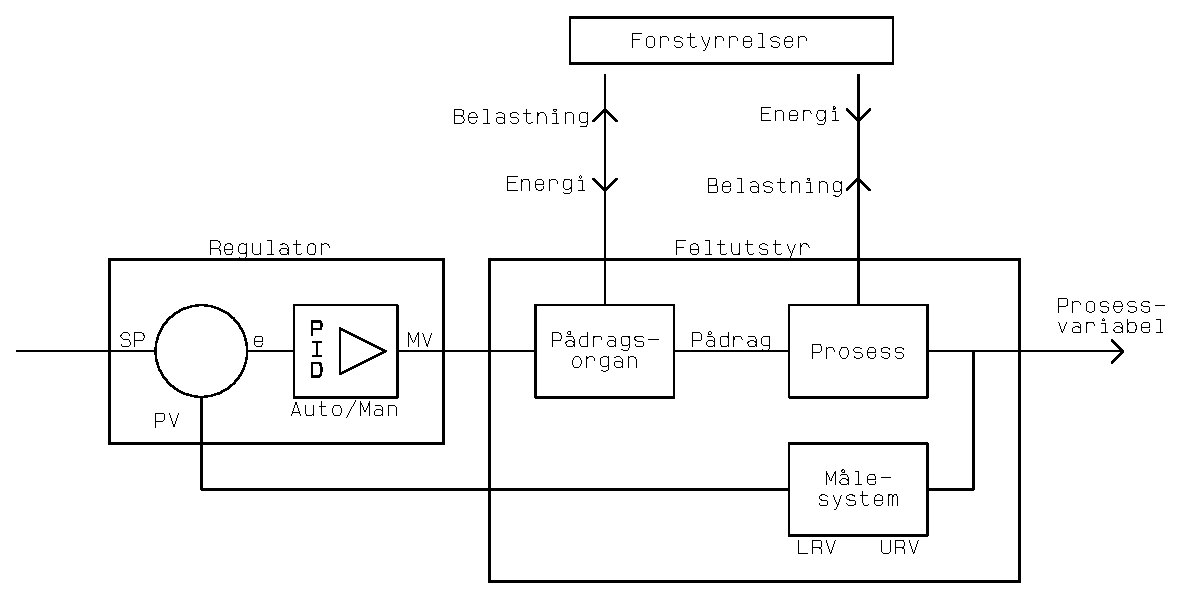
\includegraphics[width=1\textwidth]{./regblock.eps}$$

\vskip 5pt 
Direktevirkende regulator og reverstert regulator

\vskip 5pt 
En reversvirkende regulator er satt opp slik at pådraget øker når
PV er mindre enn SP. $e=SP-PV$

\vskip 5pt 
En direktevirkende regulator er satt opp slik at pådraget øker når
PV er større enn SP. $e=PV-SP$
\vfil \eject
\subsection{Optimalisering}
\subsubsection{Tims rule of tumb}
\begin{enumerate}
	\item Bare jobb med en justering av et parameter om gangen. Når du justerer flere mister du kontrollen. 
	\item Proporsjonalleddet bestemmer hvor fort en prosess går mot settpunktet. Stor proporsjonalforsterkning vil få prosesse til å nå settpunktet raskt, men du vil få et oversving og mest sannsynlig oscillasjoner. Om du setter P-forsterkningen for lavt unngår du oscillasjoner men det vil ta lang tid å nå settpunktet. Start med I-leddet og D-leddet avslått og øk forsterkningen forsiktig  fra 0.25 (0.25, 0.5, 1, 2, 4, 8, 16) til du får oscillasjoner. Reduser så forsterkningen litt. En regulator med bare P-ledd vil ha et statisk avvik fra settpunktet. 
	\item I-leddet virker ved å fjerne feil. Det kan hjelpe til med å redusere oscillasjoner og statiske avvik, men feil justering vil føre til oversving og oscillasjoner. Reduser I-tiden i forsiktig til oscillasjoner og statisk avvik er elliminert. 
	\item D-leddet er ikke nødvendig i de fleste tilfeller om det er akseptabelt med oversving. Om du trenger D-leddet øk forsiktid d-tiden til du er fornød med responsen på variasjoner i prosessen  (SP forandringer).
\end{enumerate}





\subsubsection{Ziegler\_nichols svingemetode}
\begin{enumerate}
\item Regulatoren må stå i manuell modus.
\item Få prosessen til arbidpunktet ved å justere MV manuelt eller ved å bruke en ikke optimalisert regulering. Det er viktig at PV er tilnærmet lik SP da prosessen kan ha andre egenskaper ved andre verdier. 
\item Sett regulatoren til å bare bruke P-leddet. Sett I-ledd til uendelig eller så høyt den går. NB noen regulatorer slår av I-leddet om du setter I-tiden til 0, sjekk  manualen. Sett D-leddet til 0. 
\item Sett regulatoren i automatisk modus.
\item Øk $K_p$ (du kan starte med $K_p$ = 1) inntil det oppstår stående svingninger
i sløyfen etter et sprang i settpunktet. (Reguleringssystemet er da
på stabilitetsgrensen.) Spranget skal være lite, f.eks. 5\% av referansens
verdiområde, slik at prosessen holder seg nokså nær arbeidspunktet.
Men spranget må heller ikke være så lite at responsen ikke kan observeres.
Obs: Pass på at pådraget ikke når sine metningsgrenser (maks, min)
under eksperimentene. Hvis pådraget når en av disse grensene,
vil det kunne bli stående svingninger uansett hvor stor K p vi bruker.
F.eks. kan vi da ha funnet at K pk = 1000000 gir stående svingninger,
og ihht. formelen for K p i en PI-regulator skal da K p settes lik
450000, som temmelig sikkert gir et ustabilt reguleringssystem! Det
gjelder altså å finne den minste K p u som gir stående svingninger
uten at pådraget når metningsgrensene. Dette krever at du overvåker
pådraget under eksperimentene og passer på å ikke ha så store settpunktsendringer
at pådraget når maksimum- eller minimumsverdiene.
\item Noter $K_p$ -verdien som gir stående svingninger. Denne verdien kalles
	den kritiske forsterkning $K_{Pu}$. Noter også perioden $P_u$ for de stående
svingningene. Denne perioden kalles den kritiske perioden.
\item Beregn regulatorparametrene i henhold til tabellen  og legg dem
inn i regulatoren. Forhåpentligvis får da reguleringssystemet tilfredsstillende
ytelse. Er stabiliteten i reguleringssløyfen dårlig (store oversving
i responsene), er det enklest å prøve å redusere $K_p$ .
\end{enumerate}
\begin{tabular}{|c|c|c|c|}
\hline 
 &  &  & \tabularnewline
\hline 
P-regulator & 0.5$K_{pk}$ & $\infty$ & 0\tabularnewline
\hline 
PI-regulator & 0.45$K_{pk}$ & $\frac{P_{u}}{1.2}$ & 0\tabularnewline
\hline 
PID-regulator & 0.6$K_{pk}$ & $\frac{P_{u}}{2}$ & $\frac{P_{u}}{8}=\frac{T_{i}}{4}$\tabularnewline
\hline 
\end{tabular}




\subsubsection{Skogestads metode}

Skogestad har angitt PID-regulatorinnstilling for en rekke ulike prosesstyper. Vi bruker den på følgende prosesstyper:
\begin{itemize}
\item Selvstabiliserende med tidsforsinkelse. (Eksempel på
prosess med slik dynamikk er varmeveksler.)
\item Selvstabiliserende med neglisjerbar tidsforsinkelse. Ved denne type prossess vil Z\&N være vanskelig å få til å svinge
\item Integrerende med tidsforsinkelse 
(Eksempel: Tank med transportbånd, som flistanken.)
\item Integrerende uten tidsforsinkelse (Eksempel: Væsketank styrt av pumpe eller ventil på inn- eller utløp.)
\end{itemize}

\paragraph{Innstilling av PI-regulator for tidkonstant med tidsforsinkelse}

~

\includegraphics{Sprang_selvregulerende.eps}

\[
K_{P}=\dfrac{\tau}{K\left(T_{C}+\theta\right)}
\]

\[
T_{i}=min[\tau,c(T_{c}+\theta]
\]

Her bruker en den minste verdien av $\tau$ og c (c er 2 eller 4)

\includegraphics[width=1\textwidth]{Reg_step_response01}

Her er et eksempel på en prosess med tidsforsinkelse. Når vi leser
av garfen får vi at

\begin{eqnarray*}
\theta & = & 0.5s\\
\tau & = & 5s\\
K & = & 2
\end{eqnarray*}

Det gir oss:
\[
K_{P}=\dfrac{\tau}{K\left(T_{C}+\theta\right)}=\dfrac{5}{2(0.5+0.4)}=2.5
\]

c=2 er her mindre en T=5 som gir 
\[
T_{i}=c(T_{c}+\theta)=2(0.5+0.5)=2
\]

Det gir følgende innregulering på et sprang fra 50 til 55. 

\includegraphics[width=1\textwidth]{Reg_innreg_skogestad01}

\paragraph{Innstilling av PI-regulator for integrator med tidsforsinkelse}

~

\includegraphics{Sprang_integrerendeprosess.eps}

\[
K_{i}=\dfrac{\Delta PV}{\Delta MV\cdot\Delta t}
\]

\[
Kp=\dfrac{1}{K_{i}\left(T_{c}+\theta\right)}
\]

\[
T_{i}=c\left(T_{c}+\theta\right)
\]

Eksempel:

\includegraphics[width=1\textwidth]{Reg_step_integrator}

\[
K_{i}=\dfrac{\Delta PV}{\Delta MV\cdot\Delta t}=\dfrac{40\%}{5\%\cdot8s}=1/s
\]
\[
\tau=0.5s
\]

\[
Kp=\dfrac{1}{K_{i}\left(T_{c}+\theta\right)}=\dfrac{1}{1}
\]

\[
T_{i}=c\left(T_{c}+\theta\right)=2\left(0.5+0.5\right)=2
\]
Som gir følgende innregulering

\includegraphics[width=1\textwidth]{Reg_innreg_skogestad02}
\vfil  \eject
\section{Industriroboter}
Hva er en industi robot?

\vskip 5pt 
Industrial robot as defined by iso 8373:2012:
An automatically controlled, reprogrammable, multipurpose manipulator.
Programmable in three or more axes, which can be either fixed in place or mobile for use in industrial automation applications.

\vskip 5pt 
Klassifiskajson av industriroboter ut fra mekanisk struktur. 
\begin{itemize}[noitemsep]
	\item Linære roboter (Cartesian og Gantry)
	\item SCARA robots
	\item Artikulert robot (den vi har)
	\item Parallelle roboter (delta)
\end{itemize}


Classification by mechanical structure:
Linear robots (including cartesian and gantry robots)
SCARA robots
Articulated robots
Parallel robots (delta)
Cylindrical robots
Others
Not classified
Figures 1.1 illustrates the mechanical c

\vskip 10pt 
Hva kjennetegner en industriell robot:
\begin{itemize}[noitemsep]
\item den kjører automatisk
\item den kan reprogrammeres
\item den har en arm med mer en tre akser som en kan feste ulike verktøy på
\item den kan enten stå fast eller være flyttbare
\item den er laget for å løse industrelle oppgaver 
\end{itemize}

Ulike industrielle roboter kan være:
\begin{itemize}[noitemsep]
\item Linære roboter
\item SCARA roboter
\item Parallelle roboter
\item Artikulerte roboter
\item Sylindriske roboter
\item 
\end{itemize}

\vskip 10pt 
Eksempler på industrielle bruksområder:


\begin{itemize}[noitemsep]
\item Forflytting av metall i deleproduksjon eller støyping
\item palletering
\item sveising
\item lakkering
\item pakking
\item automatisk lagersystem
\end{itemize}
\vfil  \eject
\subsection{Robotstudio}

Installasjon:
\begin{itemize}[noitemsep]
	\item Last ned installasjonsfeil fra fagbibliotek
	\item Installer robotware i fra
	\item Koble opp til lisensserver og hent ut en commuter lisens for 90 dager(max).
\end{itemize}











\section{Utstyr}
\subsection{Gand RIO-trainer}

Kortet kobles til PLS med en USB kabel og en trenger en USB til seriel
driver (CH340). 

\includegraphics[width=1\textwidth]{./GandRioTrainer.jpg}
\small
\begin{tabular}{|c|c|c|c|}
\hline 
\multicolumn{4}{|c|}{Modbus Data Table}\tabularnewline
\hline 
\hline 
IO & Tilkobling & Register & \tabularnewline
\hline 
Encoder &  & 0000H & Enkoder telleverdi\tabularnewline
\hline 
DO1 & åpen kollektor & 0001H & bit0\tabularnewline
\hline 
DO2 & åpen kollektor & 0001H & bit1\tabularnewline
\hline 
DO3 & åpen kollektor & 0001H & bit2\tabularnewline
\hline 
DO4 & åpen kollektor & 0001H & bit3\tabularnewline
\hline 
PWM1 & åpen kollektor & 0002H & AO 0 (PWM)\tabularnewline
\hline 
PWM2 & åpen kollektor & 0003H & AO 1 (PWM)\tabularnewline
\hline 
PWM3 & åpen kollektor & 0004H & AO 2 (PWM)\tabularnewline
\hline 
DI1 & 24VDC & 0005H & bit0\tabularnewline
\hline 
DI2 & 24VDC & 0005H & bit1\tabularnewline
\hline 
DI3 & 24VDC & 0005H & bit2\tabularnewline
\hline 
DI4 & 24VDC & 0005H & bit3\tabularnewline
\hline 
DI5 & 24VDC & 0005H & bit4\tabularnewline
\hline 
DI6 & 24VDC & 0005H & bit5\tabularnewline
\hline 
AI2 & 4-24mA/0-5V & 0006H & AI2\tabularnewline
\hline 
AI1 & 4-24mA/0-5V & 0007H & AI1\tabularnewline
\hline 
\end{tabular}
\normalsize
\vfil \eject
\section{Instrumenter}
\subsection{multimeter}
\subsection{loop claibrator}
\subsection{nettverkstester}
\subsection{megger}
\subsection{kontinuitetstester}





\vfil \eject
\section{Formelsamling}

\subsection{Elektroteknikk}
\vskip 2.5pt
\subsubsection*{Ohms lov}
\vskip 2.5pt
$U=R\cdot I$.
\vskip 2.5pt
\subsubsection*{Kirchoffs lover}
\vskip 2.5pt  
Strøm $\Sigma I=0$\\
\vskip 2.5pt  
$I=I_{1}+I_{2}+\cdot\cdot\cdot+I_{n}$\\
\vskip 2.5pt  
$R=\dfrac{1}{\dfrac{1}{R_{1}}+\dfrac{1}{R_{2}}+\cdot\cdot\cdot+\dfrac{1}{R_{n}}}$
\vskip 2pt
 Spenning $\Sigma U=0$\\
\vskip 2.5pt  
$U=U_{1}+U_{2}+\cdot\cdot\cdot+U_{n}$\\
\vskip 2.5pt  
$R=R_{1}+R_{2}+\cdot\cdot\cdot+R_{n}$\\
\vskip 2pt
Lederresistans: $ R=\frac{\rho\cdot l}{A}$ 
\vskip 2pt
Kortsluttningstrøm $I_{k}=\frac{E}{R_{i}+R_{ytre}}$
\vskip 2pt
Elektrisk effekt: $P=\frac{W}{t}$
\vskip 2pt  
Effektloven: $P=U\cdot I\cdot \sqrt{3} \cdot \cos \varphi$
\vskip 2.5pt  
Virkningsgrad: $\eta=\frac{P_{avgitt}}{P_{tilf\\ort}}$
\vskip 2.5pt
Synkron hastihet: $n_1=\frac{2\cdot f}{P}$
\vskip 2.5pt 
Sakking: $S=\frac{n_1-n}{n_1}$
\vskip 2.5pt 
\subsection{Reguleringsteknikk}
\vskip 2.5pt 
\subsubsection*{PID-regulator}
$MV=$\\
$K_p(e+1/TN \int e dt + TV de/dt)+BIAS$\\
\vskip 2.5pt
$Direkte e=PV-SP$\\
$Reverserende e=SP-PV$\\
\subsubsection*{Ziegler \& Nichols svingemetode}
\subsubsection*{P-regulator}
$K_p = 0.5\cdot K_u$
\subsubsection*{PI-regulator}
$K_p = 0.45\cdot K_u$\\
$T_i = 0,83\cdot T_u$\\
\subsubsection*{PID-regulator}
$K_p = 0.6\cdot K_u$\\
$T_i = 0,5\cdot T_u$\\
$T_d = 0,125\cdot T_u$\\
\vskip 2.5pt 
\subsubsection*{Prosessdynamikk}
\vskip 2.5pt 
$\theta$=døtid
\vskip 2.5pt 
$ \text{Tidskonstant finnes når} \Delta PV_{63\%}$
\vskip 2.5pt 
$\tau$=tidskonstand
\vskip 2.5pt 
$T_C$ velges lik $\theta$
\vskip 2.5pt 
\subsubsection*{Selvstabiliserende}
\vskip 2.5pt 
$K=\dfrac{\Delta PV}{\Delta MV} $
\vskip 2.5pt 
$K_p=\dfrac{\tau}{K(T_C+\theta)}$
\vskip 2.5pt 
$T_i=2(T_C+\theta)$
\vskip 2.5pt 
\subsubsection*{Integrerende}
\vskip 2.5pt 
$K_i=\dfrac{\Delta PV}{\Delta MV \cdot {\Delta t}}$
\vskip 2.5pt 
$K_p=\dfrac{1}{K_i(T_C+\theta)}$
\vskip 2.5pt 
$T_i=2(T_C+\theta)$\\
\subsection{Måleteknikk}
\subsubsection*{Kalibrering}
Feilprosent av span:\\
$Error=\frac {IUT-Standard}{Span} \cdot 100\% $\\
\vskip 2.5pt 
Skaleringsformel:
\vskip 2.5pt 
$\dfrac{x-x_{start}}{x_{range}}=\dfrac{y-y_{start}}{y_{range}}$\\
Eksempel: $\dfrac{12mA-4mA}{16mA}=\dfrac{50\%-0\%}{100\%}$
\subsubsection*{Flowmåling}
\vskip 2.5pt 
\vskip 2.5pt 
\vskip 2.5pt 
Reynoldstall: $Re=\dfrac {D \cdot v \cdot \rho}{\mu}$\\
\vskip 2.5pt 
Bernoulli's formel:\\
$z_1 \rho g + {v_1^2 \rho \over 2} + P_1 = z_2 \rho g + {v_2^2 \rho \over 2} + P_2$\\
\vskip 2.5pt 
\subsubsection*{Law of Continuity}
$\rho_1 A_1 \overline{v_1} = \rho_2 A_2 \overline{v_2} = \cdots \rho_n A_n \overline{v_n}$\\
\\
$W = \rho A \overline{v}$\\\\
$Q=A_1 \overline{v_1} = A_2 \overline{v_2}$\\

Massestrøm: $W=\frac{m}{t}$\\
\vskip 2.5pt 
Volumstrøm: $Q=\frac{V}{t}$\\
\vskip 2.5pt 
Massetetthet: $\rho=\frac{m}{V}$\\
\vskip 2.5pt 
\subsubsection*{Trykkbaserte strømningsmålere}
Måleblende: $Q=k\cdot \sqrt{\Delta p}$\\
\vskip 2.5pt 
Måleblende med varierende $\rho$: $Q=k\cdot \sqrt{\frac{\Delta p}{\rho}}$\\
\vskip 2.5pt
Kvadratrot uttrekker:\\
s = signal i prosent (0-1)\\
$s_{ut}=\sqrt{s_{inn}}$\\
\subsubsection*{Hastighetsbaserte strømningsmålere}
Turbin og Vortex:\\
$Q=kf$\\
Elektromagnetisk:\\
$E=Blv$\\
Ultralyd:\\
$Q = k {t_{up} - t_{down} \over (t_{up})(t_{down})}$\\
 
\subsection{Nivåmåling}

$P = \rho \cdot g \cdot h $\\
\subsection{Temperaturmåling}
$R_T = R_{ref}[1 + \alpha(T - T_{ref})]$\\
European $\alpha=0.00385$\\
American $\alpha=0.00392$\\
\vfil \eject
\section{Tabeller}
\includegraphics[width=1\textwidth]{002.eps}
\vfil \eject
\includegraphics[angle=90,height=1\textheight]{./chemistry12.eps}
\vfil \eject
\includegraphics[width=1\textwidth]{calibrate03.eps}
\includegraphics[width=1\textwidth]{calibrate04.eps}
\includegraphics[width=1\textwidth]{calibrate26.eps}
\includegraphics[width=0.5\textwidth]{current09.eps}
\includegraphics[width=0.5\textwidth]{current10.eps}
\includegraphics[width=0.5\textwidth]{current11.eps}
\includegraphics[width=0.5\textwidth]{current12.eps}
\includegraphics[width=0.5\textwidth]{current13.eps}
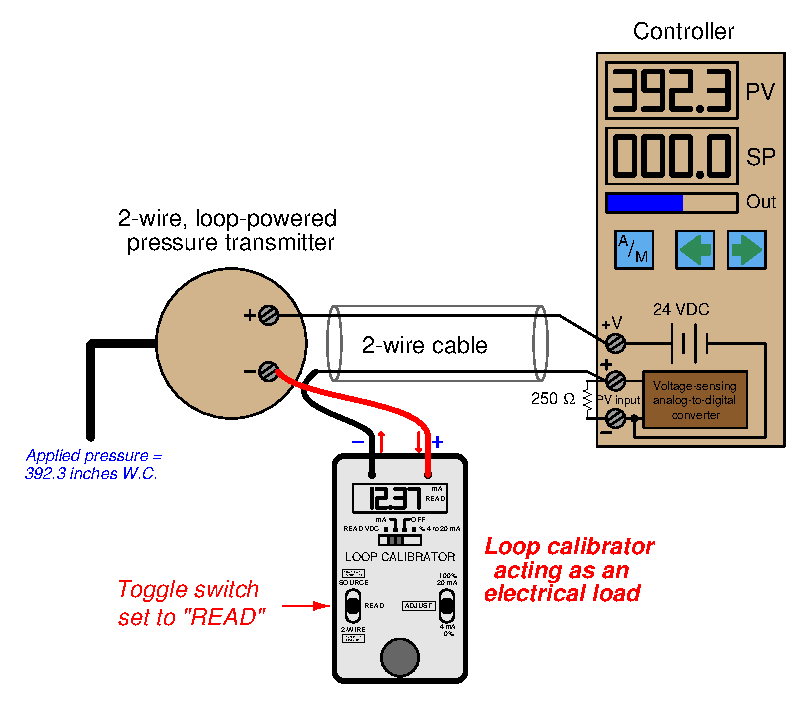
\includegraphics[width=0.5\textwidth]{current29.eps}
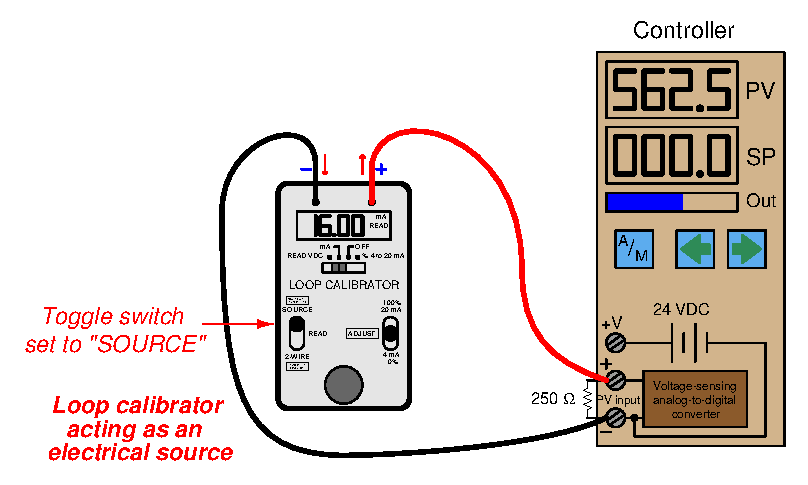
\includegraphics[width=0.5\textwidth]{current30.eps}
\includegraphics[width=0.5\textwidth]{current31.eps}
\includegraphics[width=1\textwidth]{plc_048.eps}
\includegraphics[width=1\textwidth]{plc_052.eps}
\includegraphics[width=1\textwidth]{pressure76.eps}
\end {document}
